% Copyright 2004 by Till Tantau <tantau@users.sourceforge.net>.
%
% In principle, this file can be redistributed and/or modified under
% the terms of the GNU Public License, version 2.
%
% However, this file is supposed to be a template to be modified
% for your own needs. For this reason, if you use this file as a
% template and not specifically distribute it as part of a another
% package/program, I grant the extra permission to freely copy and
% modify this file as you see fit and even to delete this copyright
% notice. 

\documentclass{beamer}
\usepackage{color}

\usetheme{Madrid}

\title[Sparse Noise]{Finding meaningful cluster structure \\ amidst background noise} % The short title appears at the bottom of every slide, the full title is only on the title page

\author[Shrinu Kushagra]
{%
  \texorpdfstring{
    \begin{columns}%[onlytextwidth]
      \column{.75\linewidth}
      \centering
      \vspace{25pt}\\ Shrinu Kushagra\\ \vspace{15pt}
      Oct 21, 2016 \\ 
      ALT 2016, Bari, Italy \\ \vspace{15pt}
      Joint work with Samira Samadi (Georgia Tech)and Shai Ben-David (University of Waterloo)
    \end{columns}
    \vspace{5pt}
	  \begin{figure}
	  
\includegraphics[trim = 0 50 0 0, clip, width=0.3\linewidth]{logo.pdf}
	  \end{figure}  
  }
  {}
}


\AtBeginSubsection[]
{
  \begin{frame}<beamer>
  \frametitle{Outline}
    \tableofcontents[currentsection]
  \end{frame}
}

\newcommand{\mc}{\mathcal}

% Let's get started
\begin{document}

\begin{frame}
  \titlepage
\end{frame}


% Section and subsections will appear in the presentation overview
% and table of contents.
\section{Introduction}

\begin{frame}{Clustering - Introduction}
  Input: $\mc X$ and $k$\\
  \begin{figure}
	  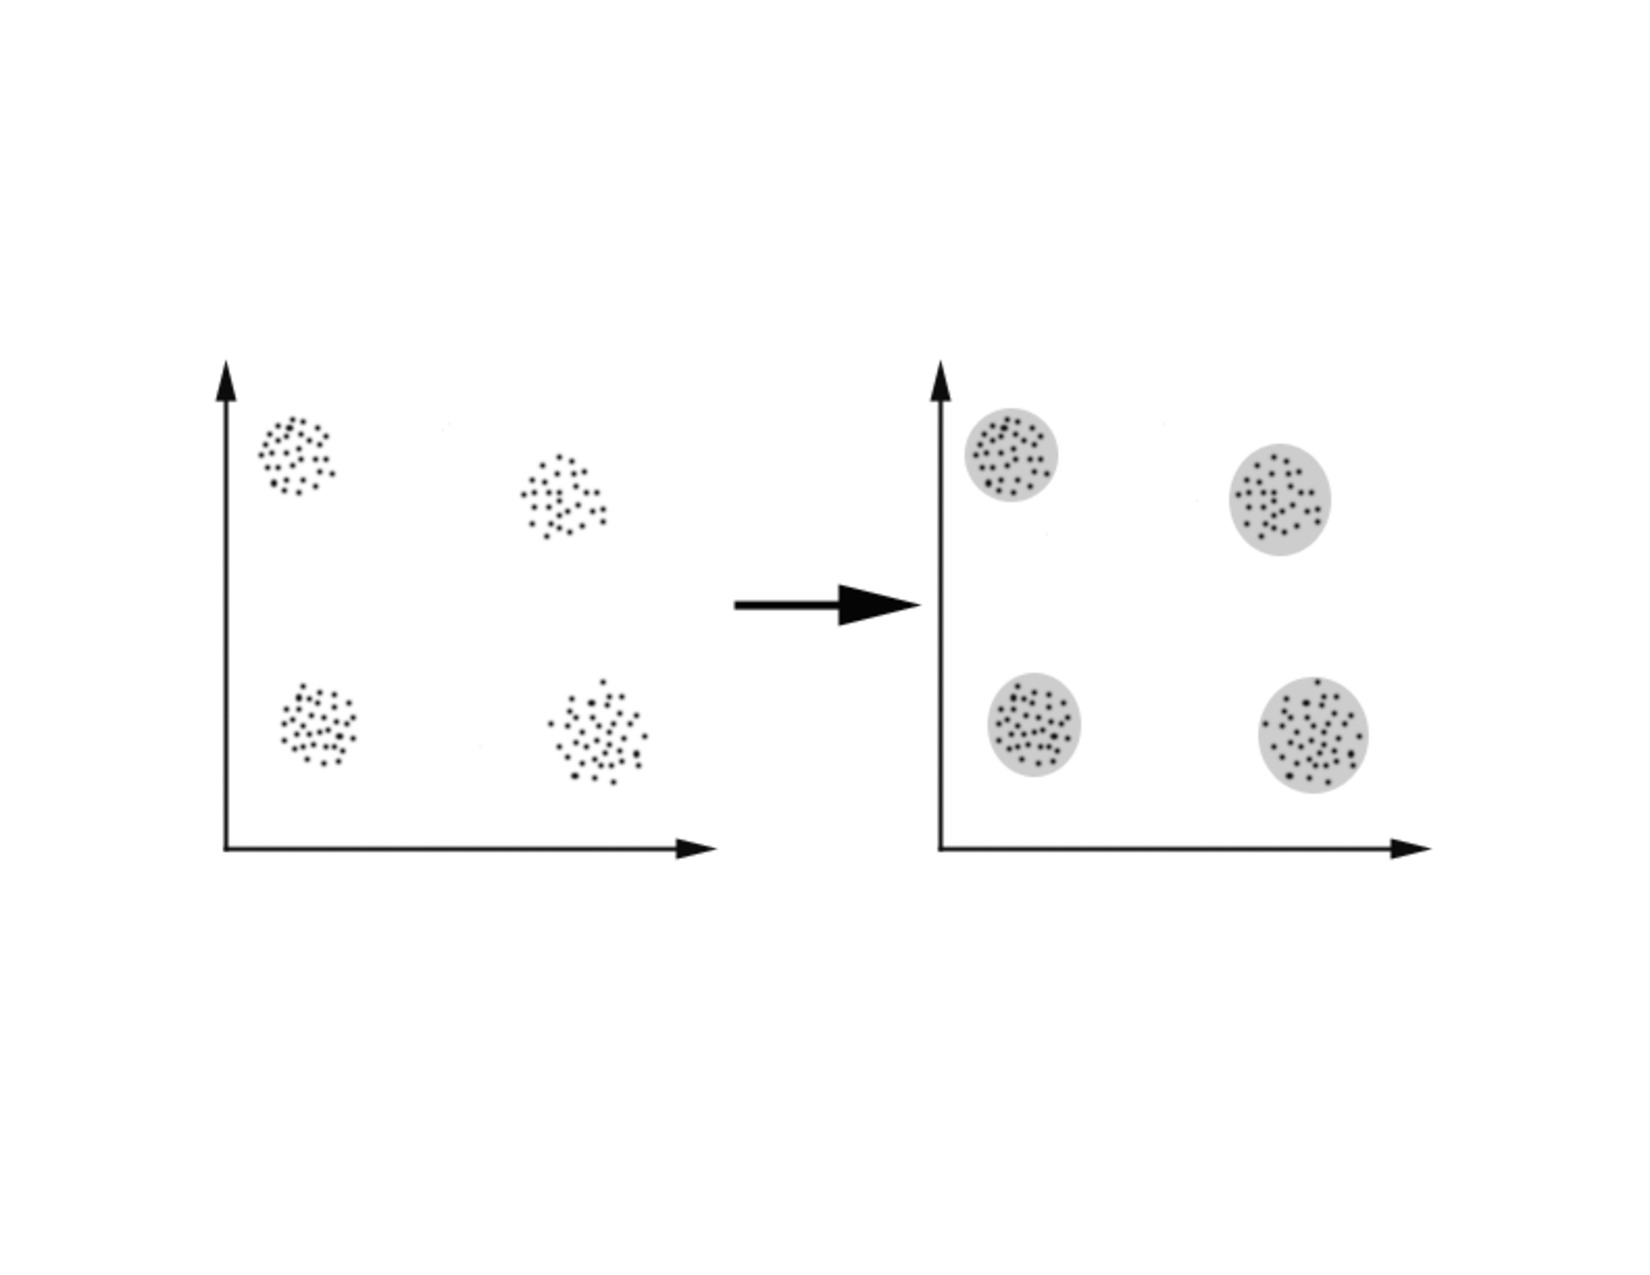
\includegraphics[trim = 50 150 50 200, clip, width=0.8\linewidth]{clustp.pdf}
	\end{figure}
	
  
  Output: Partition into $k$ clusters. $\mc C = \{X_1, \ldots, X_k\}$
\end{frame}

\begin{frame}{Clustering - Introduction}
  Most common approach
  \begin{itemize}
  	\item Associate a cost with each possible clustering $\mc C$.
  	\item Find the clustering with minimum cost. $$\min_{\mc C} \sum_{i=1}^k \sum_{x \in X_i} \|x - \mu(X_i)\|^2$$
	\item $k$-means and $k$-median 
  \end{itemize}
\end{frame}

\begin{frame}{Clustering - Challenges}  
  Computationally expensive\\
  \begin{itemize}
  	\item Minimizing objective is NP-Hard.
  \end{itemize}
  \vspace{0.1in}Multiple solutions
  \begin{itemize}
  	\item Same set can be clustered in multiple ways.
  \end{itemize}
  \vspace{0.1in}Theory vs Practice
  \begin{itemize}
	\item $k$-means successfully used on various tasks.
  \end{itemize}
  
\end{frame}

\begin{frame}{CDNM}
  
  \begin{center}Clustering is difficult only when it does not matter
  \end{center}
\end{frame}

\begin{frame}{Notions of clusterability}
   $\alpha$-center proximity\\
   $$\alpha d(x, c_i) < d(x, c_j)$$ 
   \begin{figure}
	  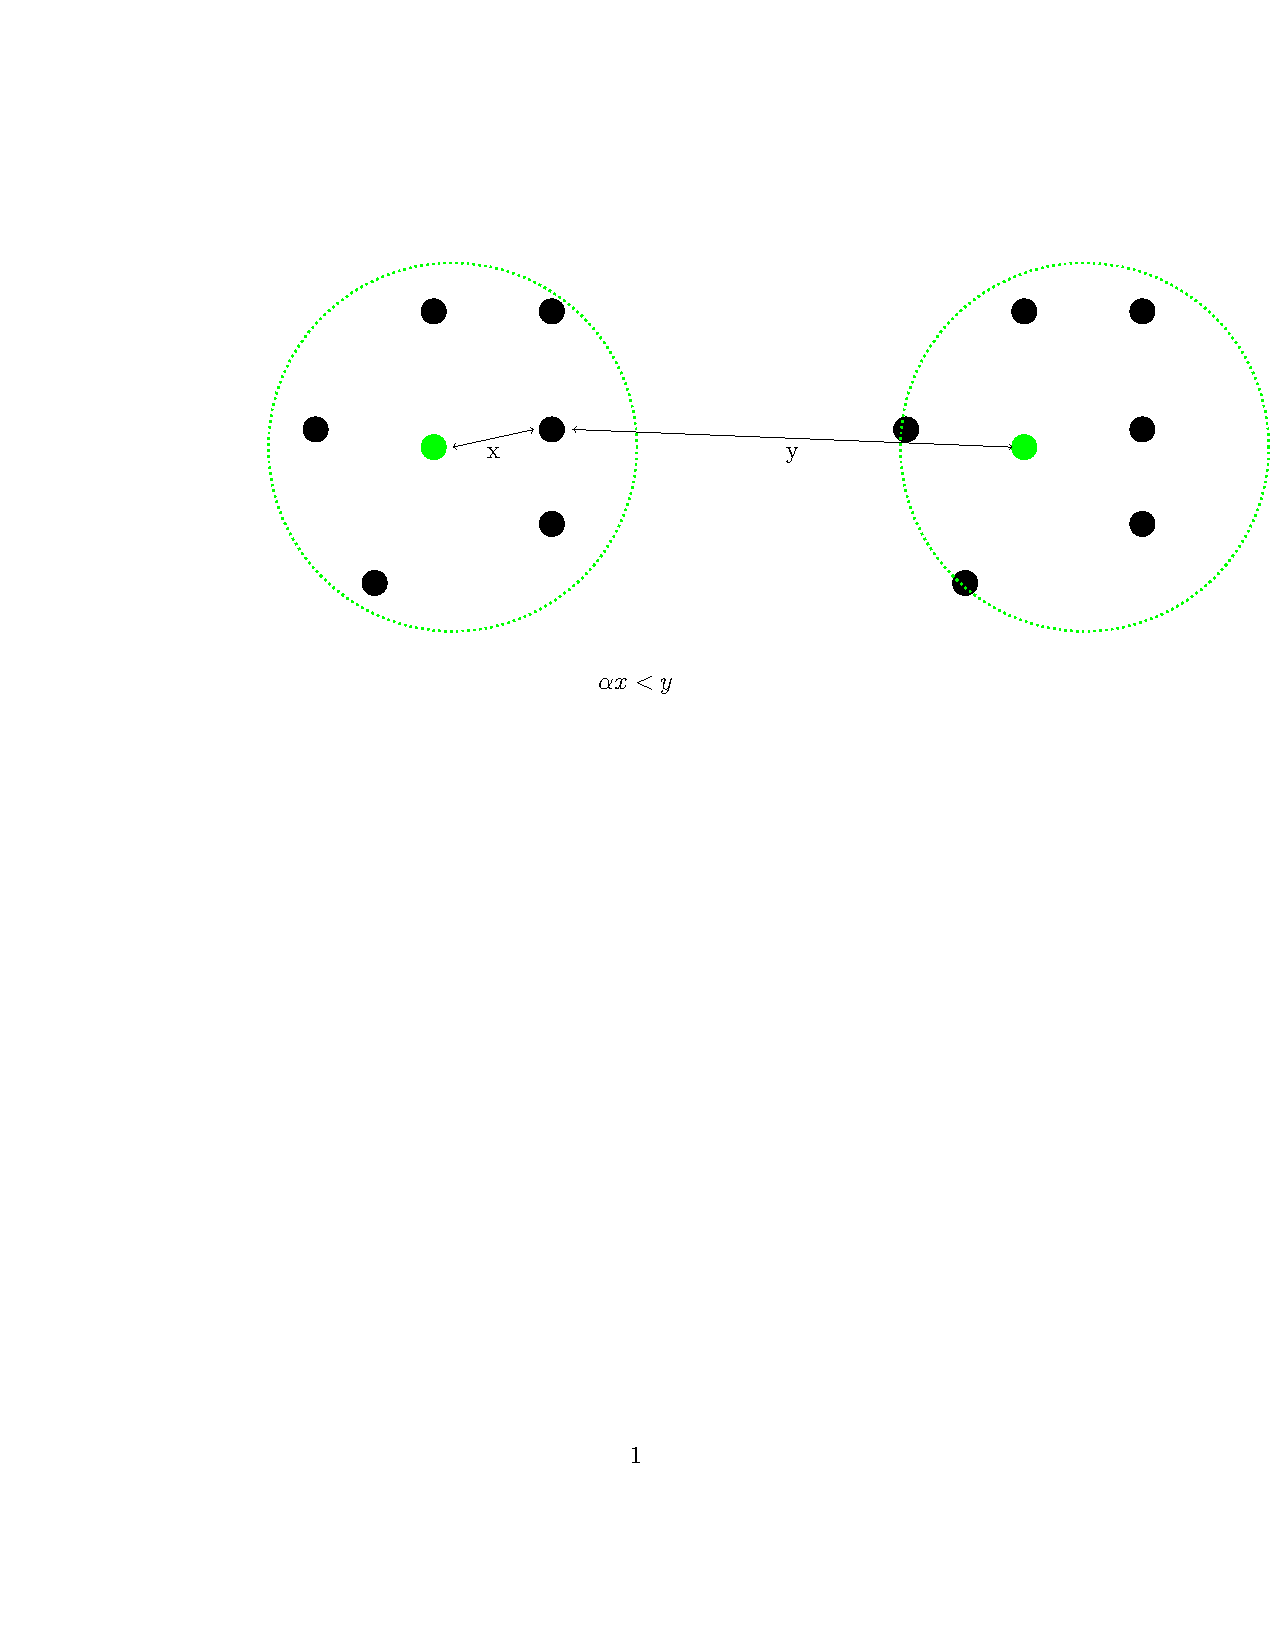
\includegraphics[trim = 0 0 0 100, clip, width=\linewidth]{figures/1.pdf}
   \end{figure}
   
\end{frame}

%\begin{frame}{Notions of clusterability}
%  \begin{itemize}
%  	\item $\alpha$-center proximity\\
%    A clustering $\mc C$ satisfies $\alpha$-center proximity w.r.t $\mc X$ if there exist centers $c_1, \ldots, c_k$  such that the following holds. For all $x \in X_i$ and $i\neq j$, $$\alpha d(x, c_i) < d(x, c_j)$$ 
%  	\item $\lambda$-center separation\\
%  	A clustering $\mc C$ has $\lambda$-center separation w.r.t $\mc X$ if there exists centers $c_1, \ldots, c_k$ such that the following holds. For all $i\neq j$, 
%  	$$d(c_i, c_j) > \lambda r(\mc C)$$
%  \end{itemize}
%\end{frame}

\section{Previous Work}

\begin{frame}{Known Results}
  
  Goal: Find the optimal $k$-median solution. $$\min_{c_1, \ldots, c_k \in \mc X} \sum_{i=1}^k \sum_{x \in X_i} \|x - c_i\|^2$$ 
  Given: Optimal solution satisfies $\alpha$-center proximity.\\
  \pause
  \vspace{0.2in}Results 
  \begin{itemize}
    \item Polytime for $\alpha > \sqrt{2}+1$ %algorithm based on finding a $k$-pruning of a hierarchical clustering tree.
    \item NP-Hard for $\alpha < 2$.  
  \end{itemize}
\end{frame}

\begin{frame}{Known Results}
  
  Goal: Find the optimal $k$-median solution. $$\min_{c_1, \ldots, c_k \in \mc X} \sum_{i=1}^k \sum_{x \in X_i} \|x - c_i\|^2$$ 
  Given: Optimal solution satisfies $\alpha$-center proximity except for an $\epsilon$ fraction of points.\\
  \pause
  \vspace{0.2in}Results 
  \begin{itemize}
    \item $(1+O(\epsilon))$-approx for $\alpha > 2+\sqrt{7} \approx 4.6$
  \end{itemize}
\end{frame}


%\begin{frame}{Known results}
%	Limitations
%	\begin{itemize}
%		\item Assumes entire set $\mc X$ has a nice structure.
%		\item Too strict. Unrealistic in pratical situations.
%	\end{itemize}
%	\vspace{0.1in}Solution
%	\begin{itemize}
%		\item Noise - Add points which do not have any structure
%	\end{itemize}
%	\vspace{0.2in}Goal: Find the optimal $k$-median solution. It is known that the optimal solution satisfies $\alpha$-center proximity except for an $\epsilon$ fraction of points. 
%  \begin{itemize}
%    \item $\alpha > 2+\sqrt{7} \approx 4.6$ - Efficient algorithm  finds a $1+O(\epsilon)$ approximation to $k$-median optimal.
%  \end{itemize}
%\end{frame}

\section{Big Picture}

\begin{frame}{Problem Setting}
  Limitations
  \begin{itemize}
  	\item Assumption on optimal %Impossible to verify - Can't find optimal solution. No way to verify if the optimal has that property.
  	\item Strict %Small noise - Upper bounded by a fraction of the dataset.  
  \end{itemize}
\end{frame}

\begin{frame}{Problem Setting}
  Our framework
  \begin{itemize}
  	\item Efficient representation of all nice solutions.
  	\item Noise is structureless.
  \end{itemize}
\end{frame}

\begin{frame}{Clustering tree}
	\begin{figure}
	  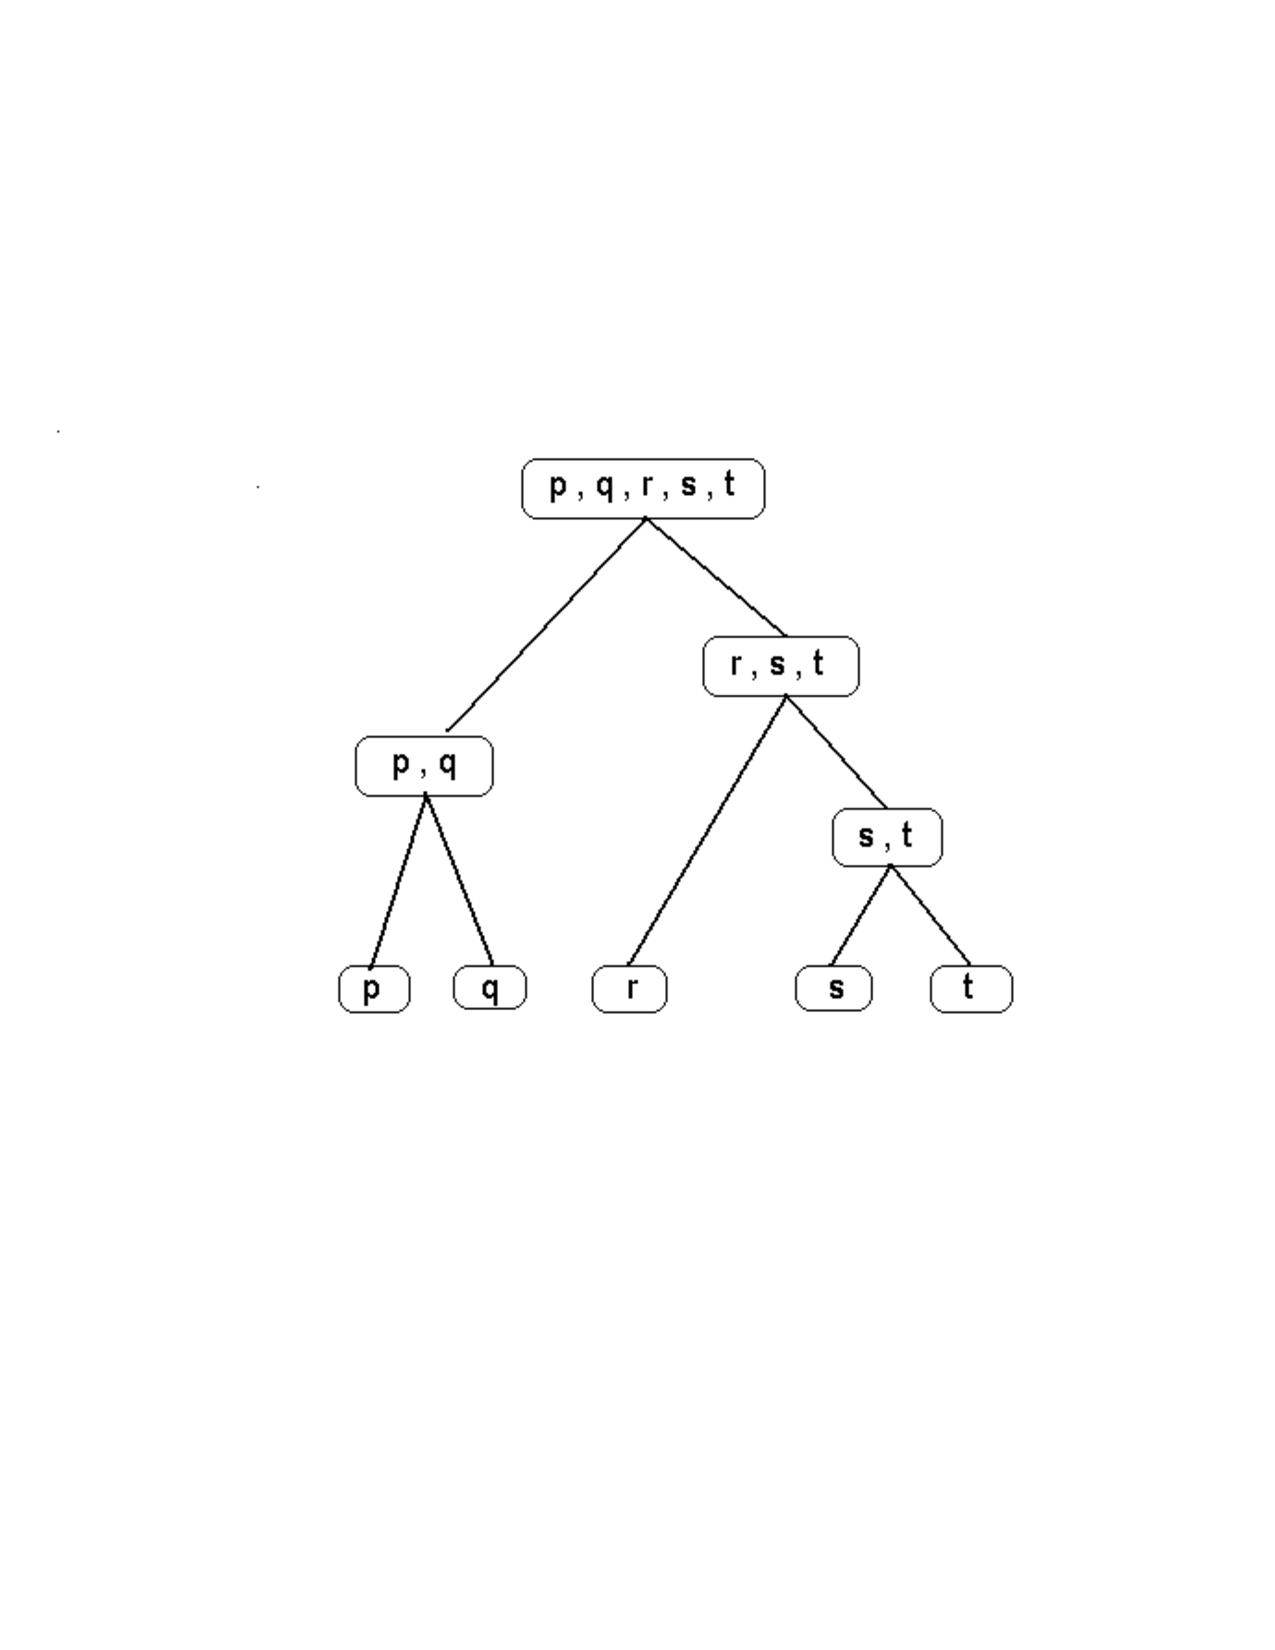
\includegraphics[trim = 50 150 50 200, clip, width=0.8\linewidth]{hier.pdf}
	\end{figure}
	\vspace{-1in}Example 3-clusterings $\{\{p\}, \{q\}, \{r, s, t\}\}$ and $\{\{p, q\}, \{r\}, \{s, t\}\}$
\end{frame}

\begin{frame}{Sparse noise}
    Any ball of small radius contains few points from $\mc X$.
    \begin{figure}
	  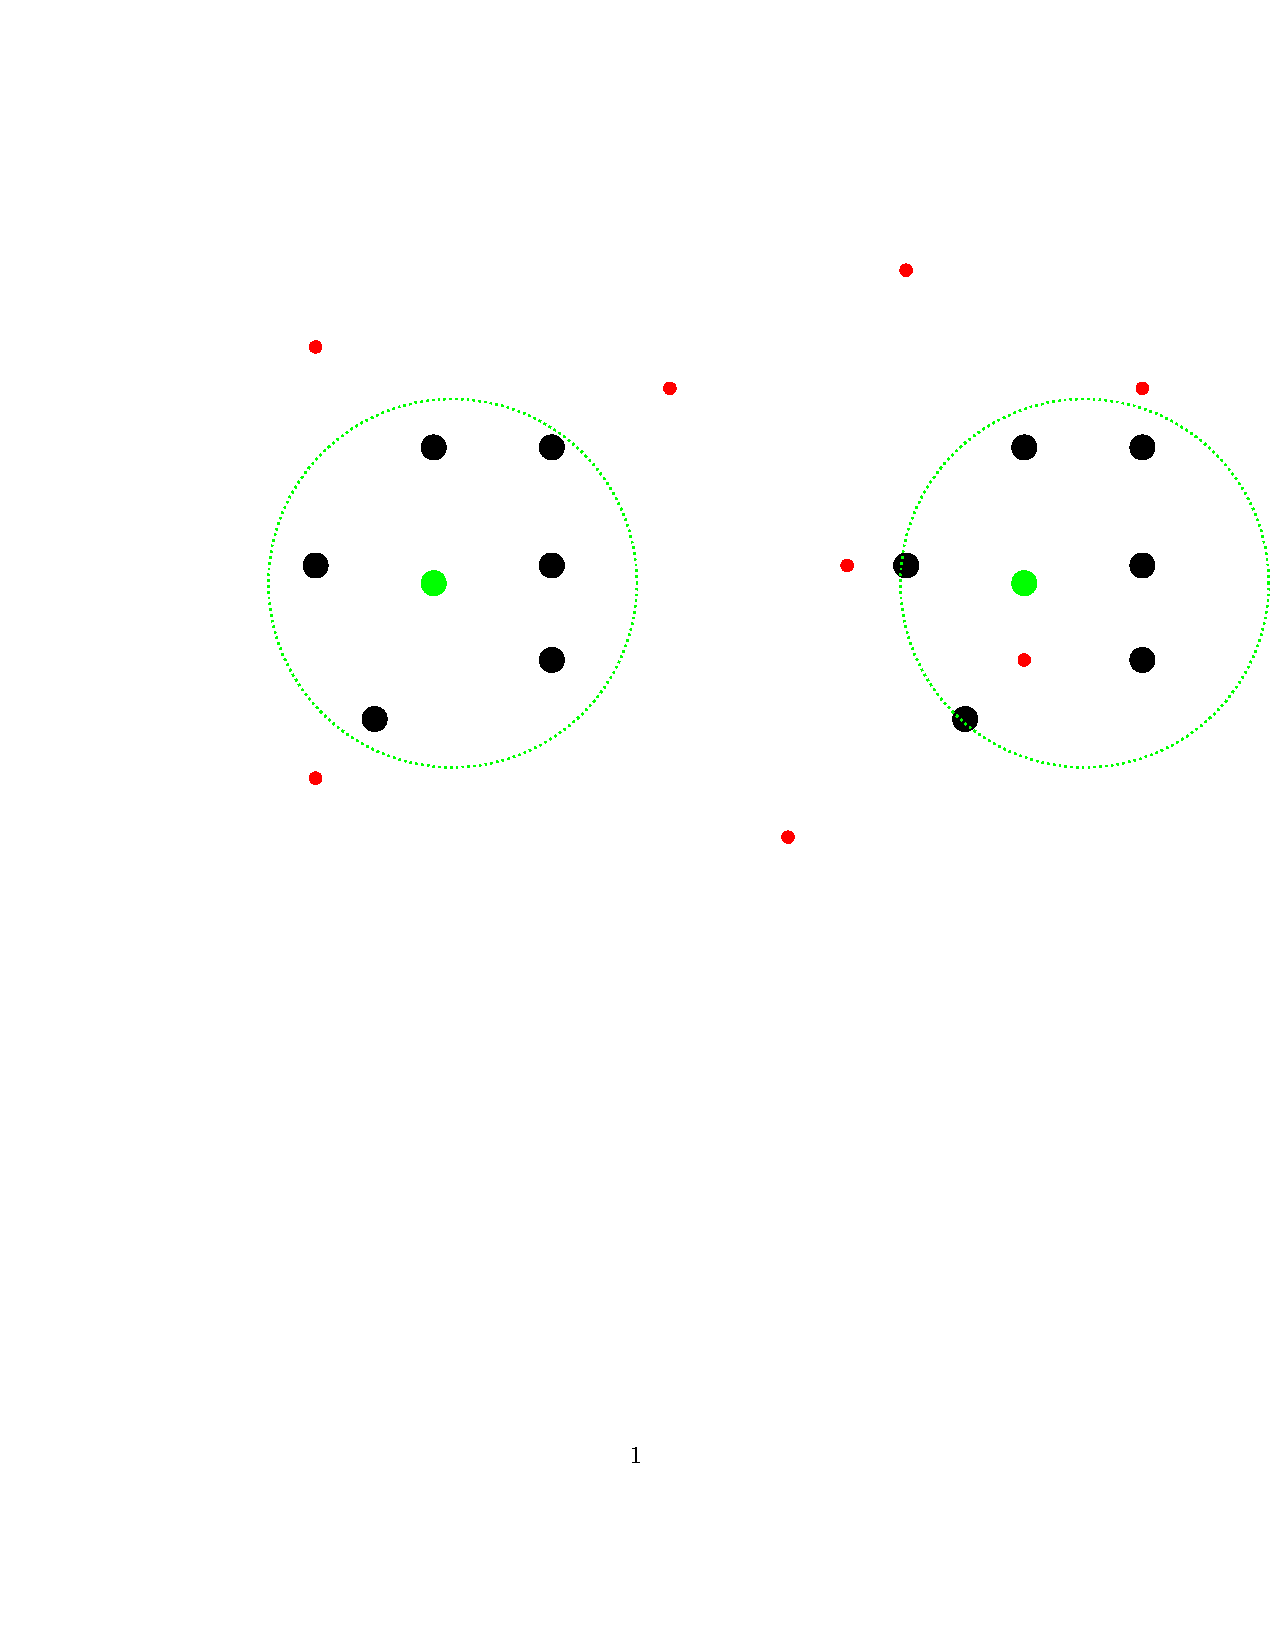
\includegraphics[trim = 100 0 0 100, clip, width=\linewidth]{figures/2.pdf}
   \end{figure}
    	 
	\textcolor{red}{Add figure}
\end{frame}

\section{Preliminaries}

\begin{frame}{Definition}
	\begin{block}{($\alpha, \eta$)-center proximity}
	Given $\mc S \subseteq \mc X$
	\begin{itemize}
  	\item[$\diamond$] $\mc S$ has {\bf $\alpha$-center proximity}
	\item[$\diamond$]$\mc X \setminus \mc S$ is {\bf $\eta$-sparse}
	\end{itemize}
	\end{block}
\end{frame}

\section{Algorithmic Approach}

\begin{frame}{Results}
  \begin{itemize}
  	\item $\alpha < 5.8$ and noise is small (but adverserial)\\ \textcolor{red}{No efficient representation}. 
  	\pause
  	\item $\alpha > 4.6$ and noise is sparse\\ 
  	\textcolor{green}{Clustering tree in poly time}.
  	\pause
  	\item $\alpha < 4.4$ and noise is sparse\\ 
  	\textcolor{red}{No efficient representation}. 
  \end{itemize}
\end{frame}

\begin{frame}{Clustering under $(\alpha, \eta)$-center proximity}
	\begin{block}{The algorithm}
	  Input: $(\mc X, d)$ and a parameter $t$.\\
	  Output: A hierarchical clustering tree.\\
	  \vspace{0.1in}Initialize every point in its own cluster.\\
	  Go over all pairs of points $p, q$ in increasing order of distance.\\
	  If $B := B(p, d(p, q))$ satisfies the sparse-distance condition
	  \begin{itemize}
	  	\item Merge all clusters that intersect with $B$ into a single cluster
	  \end{itemize}
    \end{block}
        
    \vspace{0.2in}We say that the ball $B$ satisfies the sparse distance condition w.r.t clustering $\mc C$ when the following holds.
	\begin{itemize}
	  \item $|B| \ge t$.
	  \item For any $X_i \in \mc C$, if $X_i \cap B \neq \emptyset$, then $X_i \subseteq B$ or $|B \cap X_i| \ge t/2$.
	\end{itemize}
\end{frame}

\begin{frame}{Satisfies sparse-distance}
   \begin{figure}
	  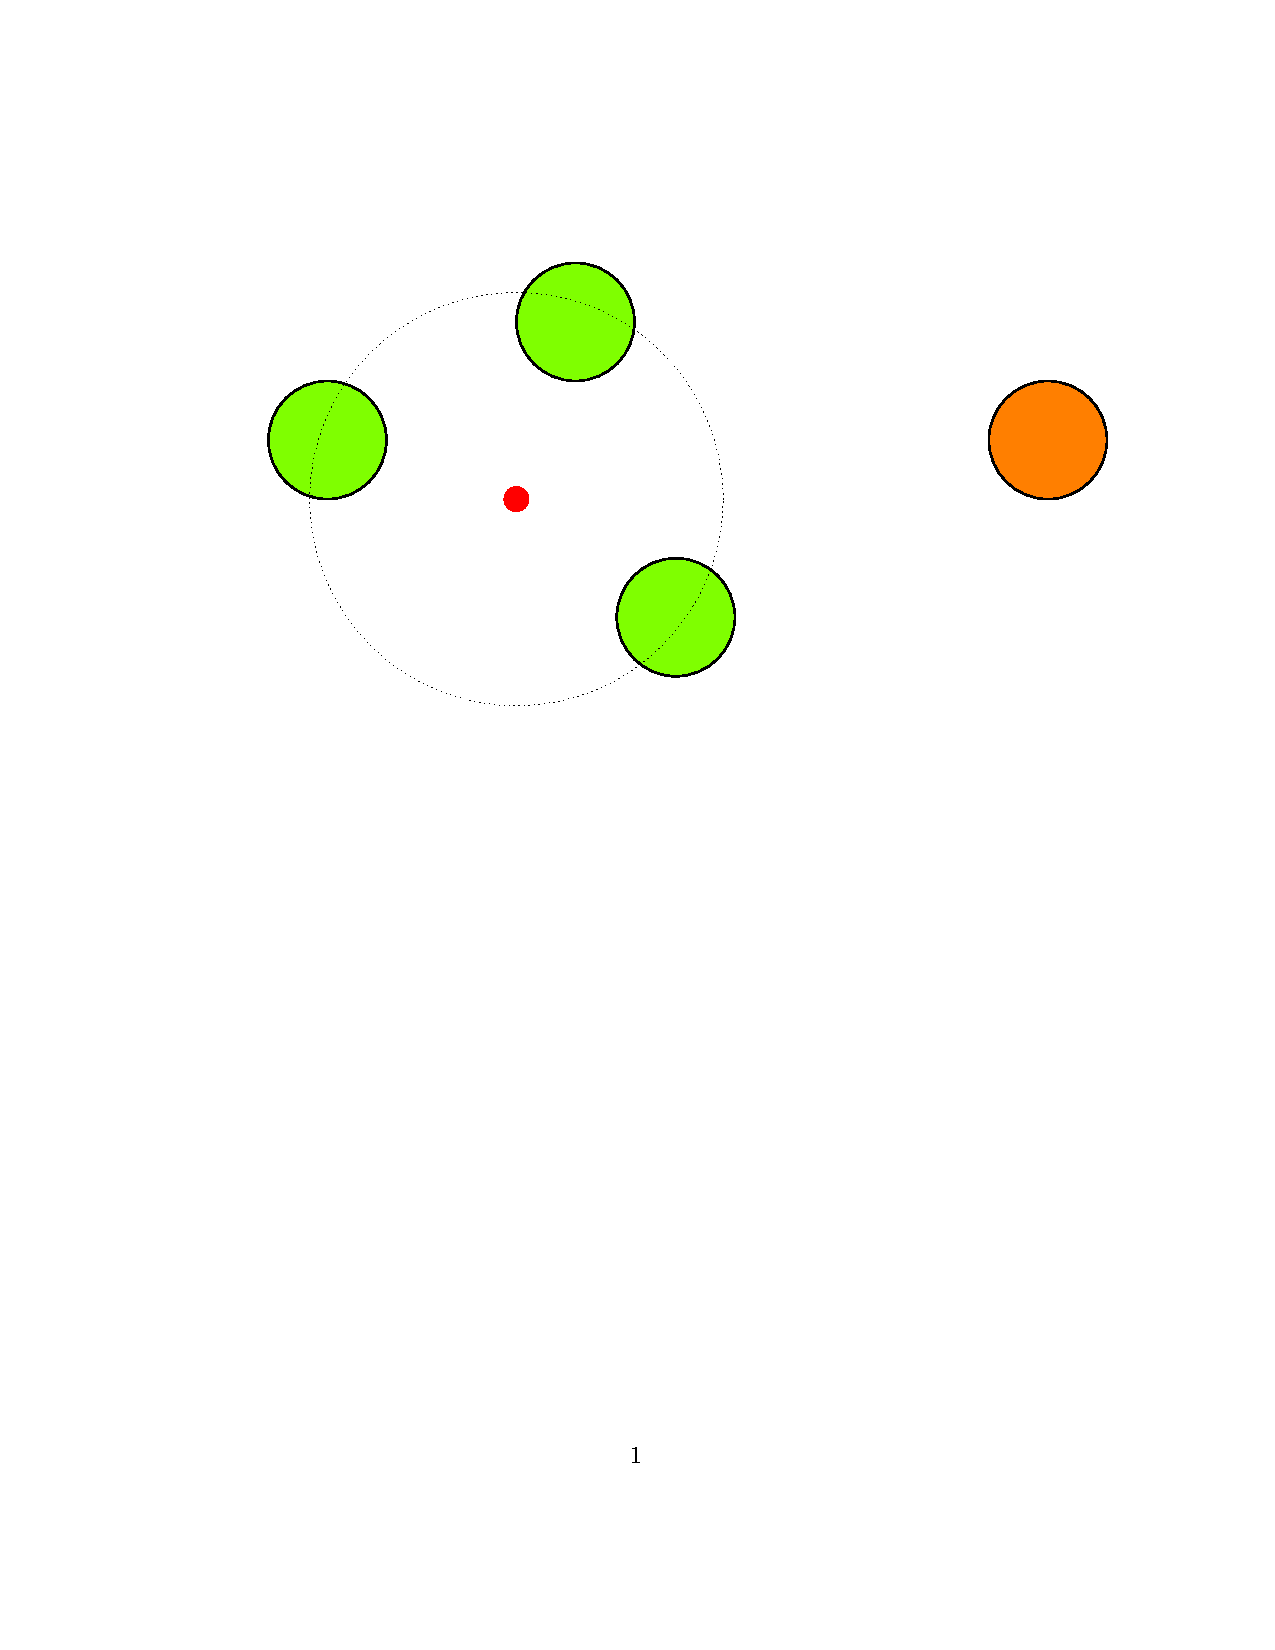
\includegraphics[trim = 100 0 0 100, clip, width=\linewidth]{figures/3.pdf}
   \end{figure}
\end{frame}
\begin{frame}{Doesn't satisfy sparse-distance}   
   \begin{figure}
	  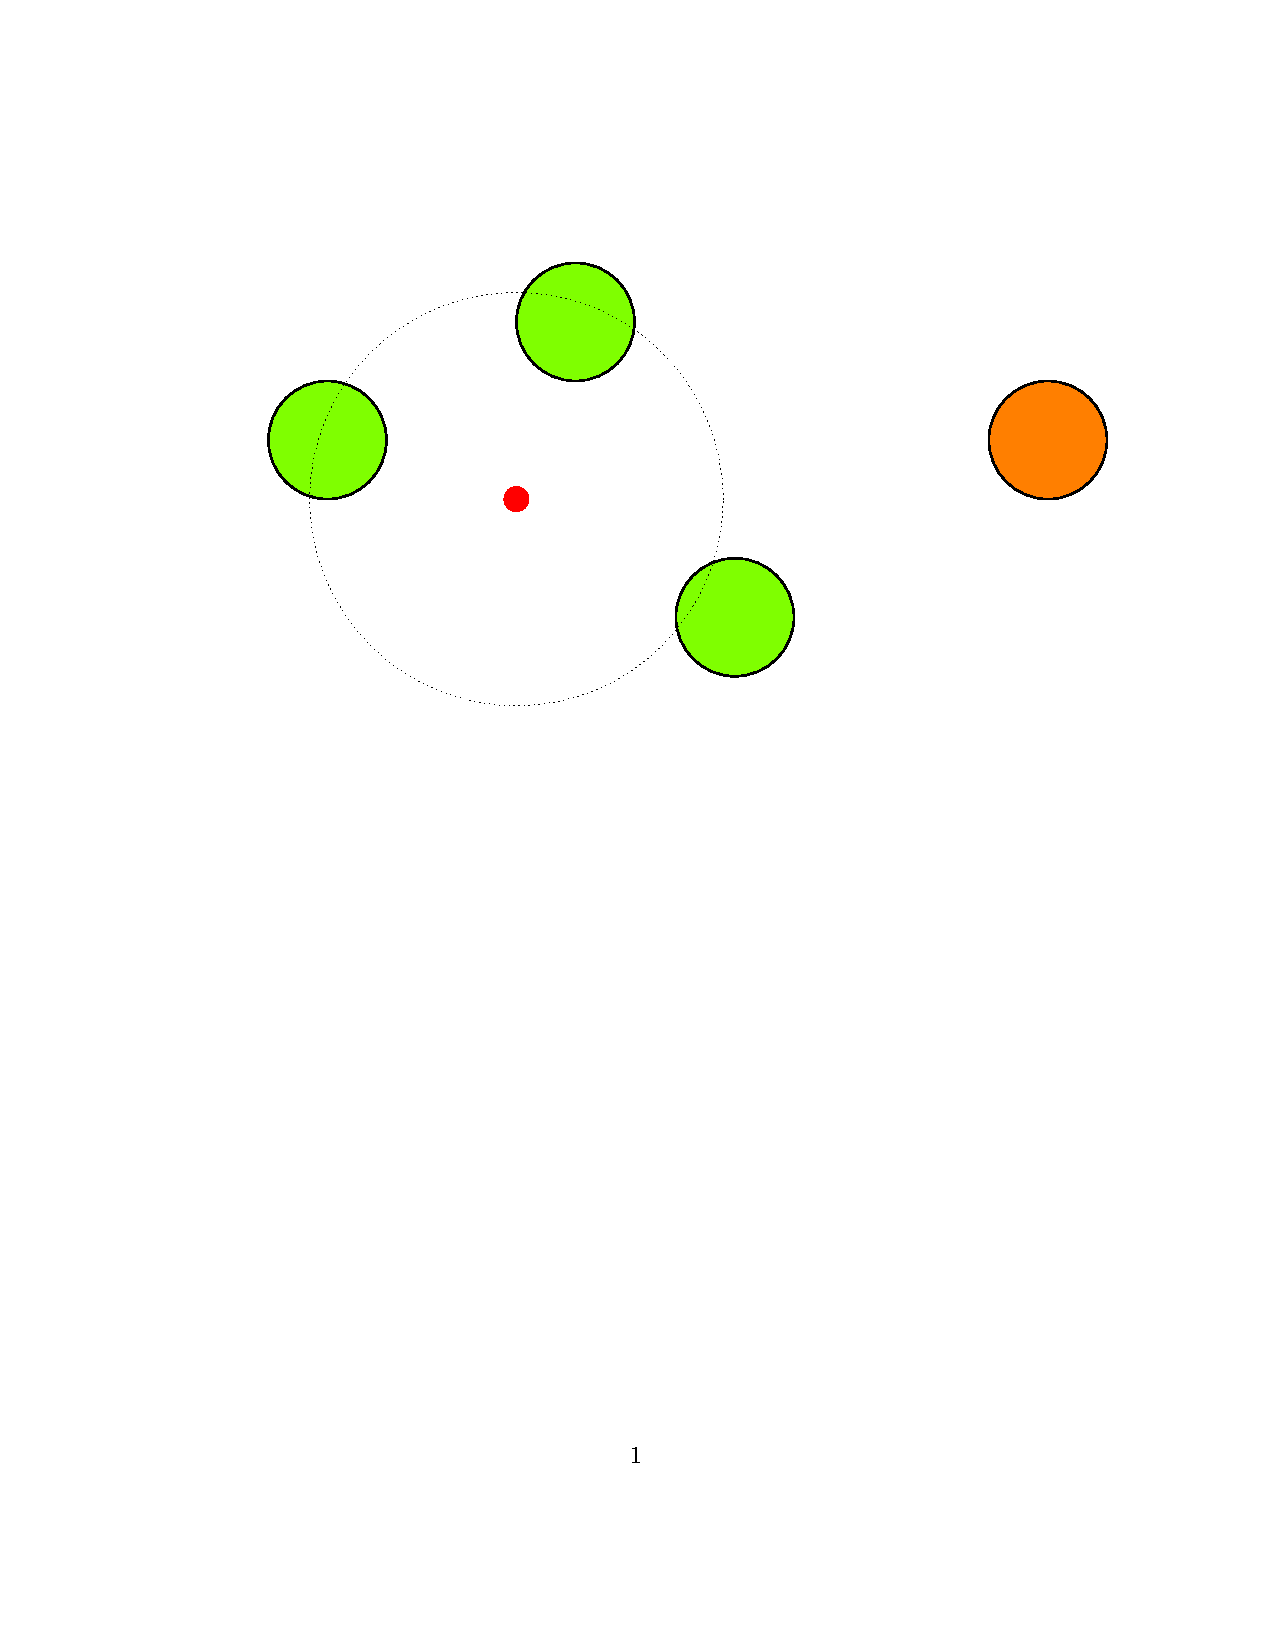
\includegraphics[trim = 100 0 0 100, clip, width=\linewidth]{figures/4.pdf}
   \end{figure}
\end{frame}

\begin{frame}{Lower bound}
	If $\alpha < 3 + \sqrt{2}$ and noise is sparse, then there doesn't exist a clustering tree which can capture all nice solutions.
	\begin{figure}[!t]
	  \begin{center}
	    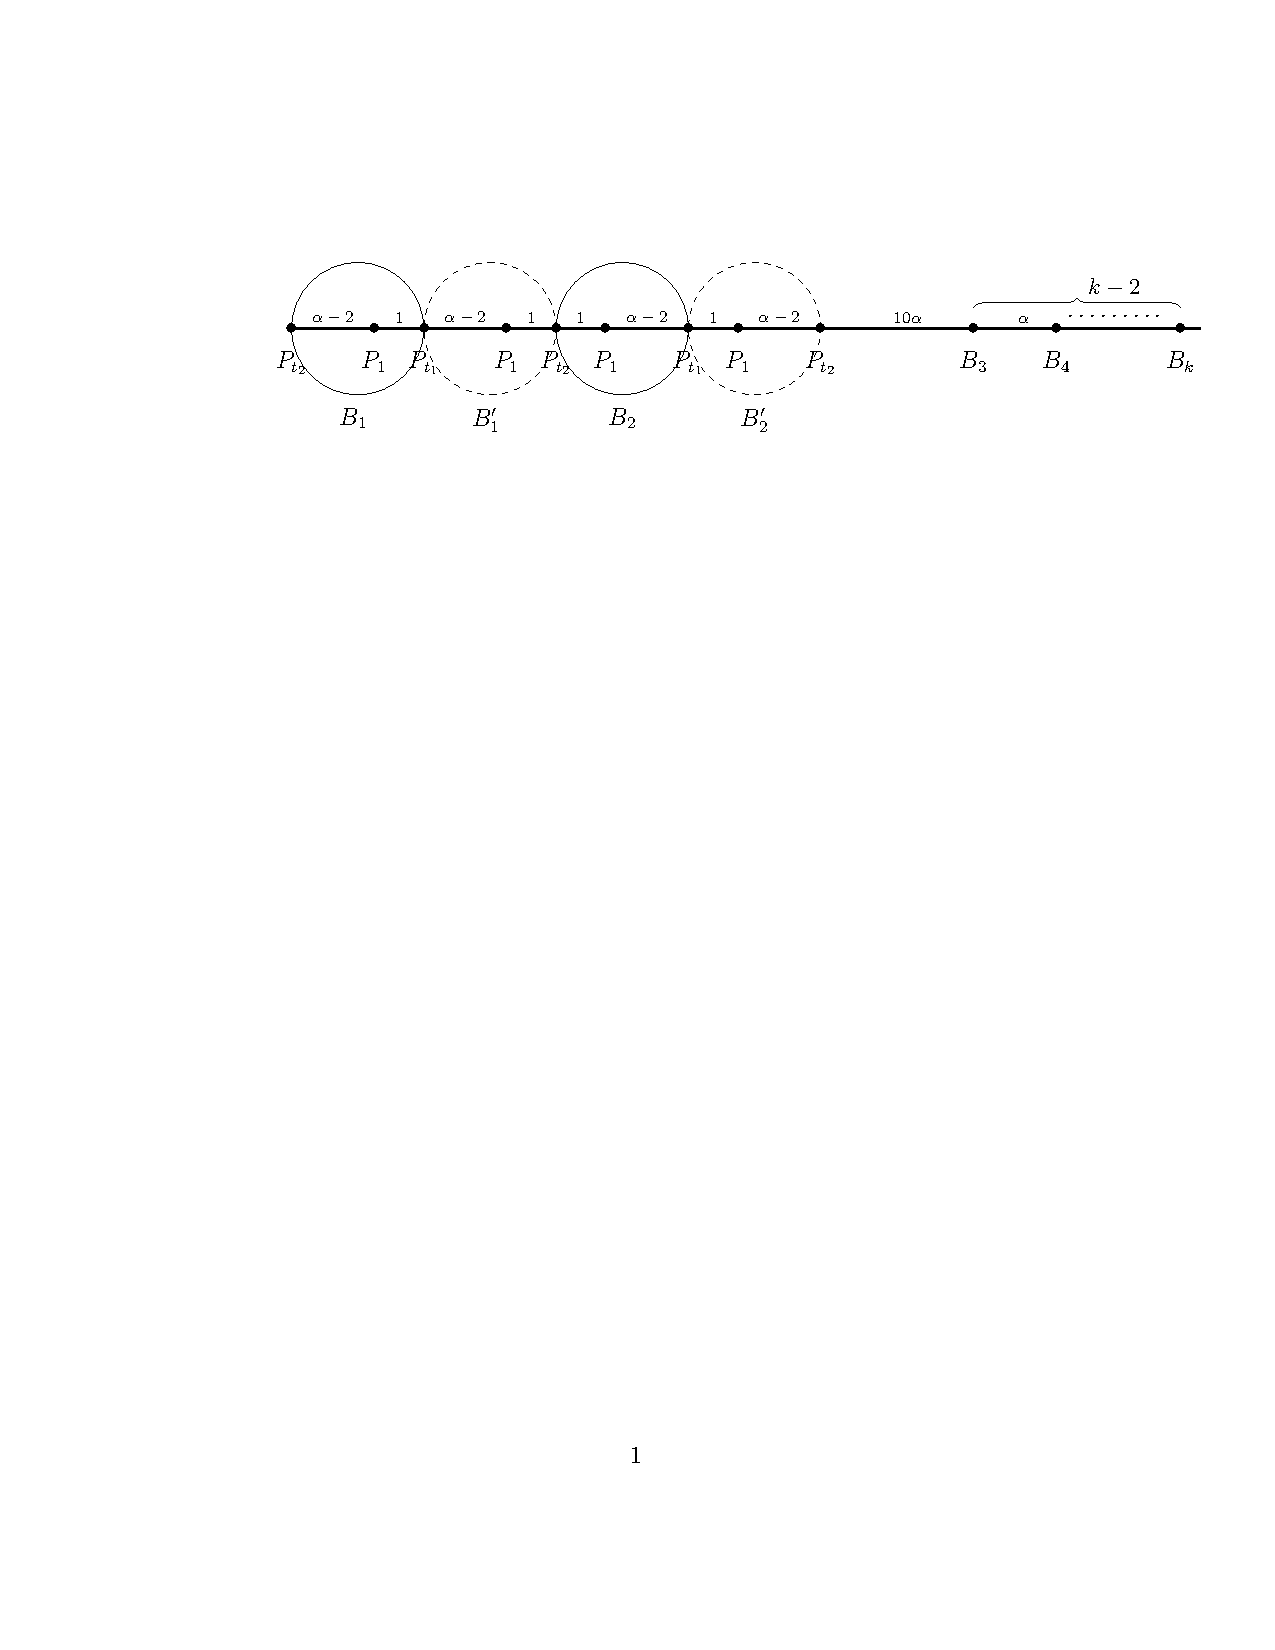
\includegraphics[trim={47mm 205mm 12mm 44mm},clip,width=\textwidth]{lbdFig2.pdf}
	  \end{center}
	\end{figure}
	Same ideas can be extended to a list output. Any list should have size $> 2^{k/2}$
\end{frame}

\begin{frame}{Justification of sparse noise}
    \begin{itemize}
	  \item Data $\mc S$ has nice structure.
	  \item Noise $\mc N$ is added by a non-concentrated distribution.
	  \pause
	  \item $\mc X = \mc S \cup \mc N$ satisfies the structureless noise definition with high probability.
    \end{itemize}
\end{frame}

\begin{frame}
    \Huge{\centerline{Thank You!}}
\end{frame}

%----------------------------------------
%        Figure Samples
%----------------------------------------

% All of the following is optional and typically not needed. 
\appendix
\section<presentation>*{\appendixname}
\subsection<presentation>*{For Further Reading}

%\begin{frame}[allowframebreaks]
  %\frametitle<presentation>{For Further Reading}
   % 
  %\begin{thebibliography}{10}
    
  %\beamertemplatebookbibitems
  % Start with overview books.

  %\bibitem{Author1990}
   % A.~Author.
    %\newblock {\em Handbook of Everything}.
    %\newblock Some Press, 1990.
 
    
  %\beamertemplatearticlebibitems
  % Followed by interesting articles. Keep the list short. 

  %\bibitem{Someone2000}
   % S.~Someone.
    %\newblock On this and that.
    %\newblock {\em Journal of This and That}, 2(1):50--100,
    %2000.
  %\end{thebibliography}
%\end{frame}

\end{document}


